% ===============================================================================
% = LaTeX Beamer Template des Arbeitsbereichs Sicherheit in verteilten Systemem
% = (c) 2012 Prof. Dr. Hannes Federrath, Uni Hamburg, Fachbereich Informatik
% = http://www.informatik.uni-hamburg.de/svs/
% ===============================================================================
%
\documentclass[t]{beamer}
% Option t              Place text of slides at the (vertical) top of the slides.
% Option handout        Ein PDF ohne Pausen und Overlayeffekte erzeugen.
% Option aspectratio=43 169 => 16:9, 1610 => 16:10, 43 => 4:3
\usepackage[utf8]{inputenc}
\usepackage[ngerman]{babel}
\usepackage{graphicx,xcolor}
\usepackage[T1]{fontenc} % 8-Bit-Zeichen; ermöglicht korrektes Kopieren von Umlauten aus dem pdf
\usepackage[scaled]{helvet}

\usepackage{beamerthemedefault}

% Ränder definieren
\setbeamersize{text margin left=5ex, text margin right=5ex}

% Farbdefinitionen
\definecolor{svsgrau1}{RGB}{191,191,191} % Balken in Kopfzeile
\definecolor{svsgrau2}{RGB}{123,123,123} % Folienüberschriften
\definecolor{svsrot}{RGB}{255,0,0} % Bullets
\definecolor{svshellblau1}{RGB}{153,204,255} % Block Hintergrund
\definecolor{svshellblau2}{RGB}{24,113,248} % Anstrich Ebene 2
\definecolor{svsdunkelblau}{RGB}{38,82,128} % Text der Ebene 1

% Navigationsleiste ausblenden
\beamertemplatenavigationsymbolsempty

% Farben der Bullets der Ebenen
\setbeamercolor{itemize item}{fg=svsrot}
\setbeamercolor{itemize subitem}{fg=svshellblau2}
\setbeamercolor{enumerate item}{parent=itemize item}
\setbeamercolor{enumerate subitem}{parent=itemize subitem}

% Formen der Bullets der Ebenen
\setbeamertemplate{itemize item}[circle]
\setbeamertemplate{itemize subitem}{--}
\setbeamertemplate{itemize subsubitem}[circle]

% Farben der Texte
\setbeamercolor{title}{fg=black}
\setbeamercolor{structure}{fg=svsgrau2}
\setbeamercolor{section in toc}{fg=black}
\setbeamercolor{framesubtitle}{fg=svsdunkelblau}
\setbeamercolor{itemize/enumerate body}{fg=svsdunkelblau}
\setbeamercolor{itemize/enumerate subbody}{fg=black}
\setbeamercolor{itemize/enumerate subsubbody}{fg=black}

% Zeichensätze der Texte
\setbeamerfont{author}{size=\normalsize}
\setbeamerfont{institute}{size=\normalsize}
\setbeamerfont{date}{size=\normalsize}
\setbeamerfont{frametitle}{size=\large}
\setbeamerfont{framesubtitle}{size=\footnotesize\raggedleft}
\setbeamerfont{sections/subsections in toc}{size=\normalsize}
\setbeamerfont{itemize/enumerate body}{size=\normalsize}
\setbeamerfont{itemize/enumerate subbody}{size=\normalsize}
\setbeamerfont{itemize/enumerate subsubbody}{size=\normalsize}

% Definitionen für farbig hinterlegten Block
\setbeamertemplate{blocks}[rounded]
\setbeamercolor{block title}{fg=black,bg=svshellblau1}
\setbeamercolor{block body}{parent=normal text,use=block title,bg=block title.bg!25!bg}
\setbeamerfont{block title}{size=\normalsize}
\setbeamerfont{block body}{size=\normalsize}

% Definitionen für Agenda (FIXME: noch stärker an normale Listendefs. anpassen)
\setbeamertemplate{section in toc}[sections numbered]
\setbeamertemplate{subsection in toc}[square]

% Kopfzeile
\setbeamertemplate{headline}{
	
\includegraphics[height=8mm]{pic/UHH-Logo_2010_ohneText.png}%
	\color{svsgrau1}\rule{\paperwidth}{8mm}\newline
	\mbox{}\rule{1em}{0pt}\rule{0pt}{8ex}
	\dotfill\newline\vspace{-7.3ex}
}

% Fusszeile
\setbeamertemplate{footline}[text line]{
	\parbox[b]{50mm}{\insertframenumber\\[1ex]}
}

% Hintergrund Titelseite
\defbeamertemplate{background canvas}{titlepage}{%
	{\color{svsgrau1}\vrule width\paperwidth height0.7\paperheight}%
	{\color{white}\vrule width\paperwidth height0.3\paperheight}%
}

% =============================
% = Ab hier Inhalte ändern...
% =============================

\title{IT-Sicherheit und Schutz vor Malware im Automobil}
\author[Beer, Grusche, Stock]{Arne Beer, Stefan Grusche, Joshua Stock}
% \institute[Uni Hamburg]{Universität Hamburg\\ Fachbereich Informatik}
\date{}

\begin{document}

\begingroup
	\setbeamertemplate{background canvas}[titlepage]
	\begin{frame}[plain]
		\vskip8mm
		
\includegraphics[width=2.2cm]{pic/svs_logo_hires-ohne-was.png}
		% \vskip-20mm % dies geht nur bei kurzen Vortragstiteln
		\titlepage
		\vspace{\fill}
		
\includegraphics[width=2.9cm]{pic/UHH-Logo_2010_Farbe_RGB_hires_nomargin.png}
		\vskip20pt
	\end{frame}
\endgroup

\begin{frame}{Gliederung}
	\tableofcontents
\end{frame}

\section{Can Bus} % erscheint in Agenda
\begin{frame}
	\frametitle{CAN-Bus: Was ist der CAN-Bus}
	\begin{itemize}
		\item
	    %
  	    \item
  	    %
	\end{itemize}

\end{frame}

\section{Ausgewählte Angriffsvektoren} % erscheint in Agenda
\begin{frame}
	\frametitle{Angriffsvektoren: verwundbare Komponenten am CAN-Bus}
    \begin{center}
    	\begin{figure}
			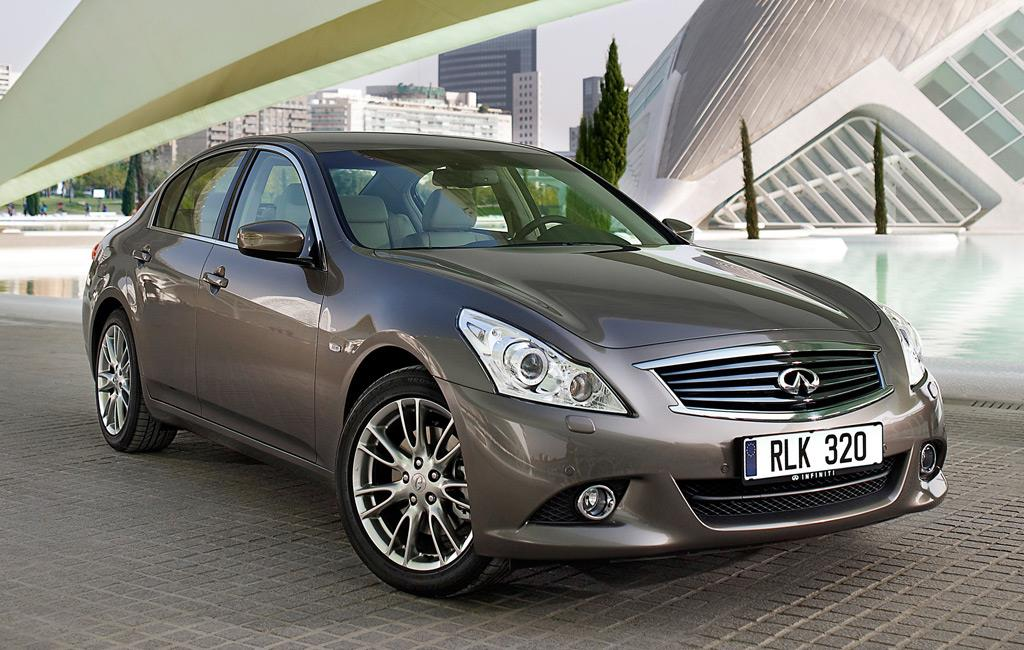
\includegraphics[width=0.3\textwidth]{pic/remote_attack_images-026.jpg} \ \
			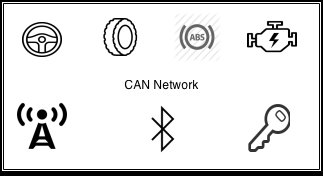
\includegraphics[width=0.3\textwidth]{pic/remote_attack_images-027.jpg}
      	  	\caption[2010 Infiniti G37 (Sedan)]{Sedan Infiniti (2010) und Komponenten im CAN-Netzwerk}
			% Lenkradkontrolle, Reifendrucksensoren, Bremssysteme, Motorkontroll-Einheit, AM/FM-Radio, Bluetooth, ferngesteuertes Öffnen bzw. Starten des Autos
			\cite{Quellen}
			%Quellen für Bilder:
			% http://images.thecarconnection.com/lrg/2010-infiniti-g37-sedan_100234015_l.jpg
			% [MV14]
		\end{figure}
	\end{center}
	\begin{itemize}
		\item (zu) offene Schnittstellen
	    %z.B. Update über Internet ohne sichere Authentifizierung
  	    \item Redundanzen in der Implementierung
  	    %z.B. muss Bluetooth-Modul Zugriff auf den Bus haben?
	\end{itemize}
\end{frame}

 \subsection{Mobilfunk} % erscheint in Gliederung
 \begin{frame}
	\frametitle{Mobilfunk I}
        \begin{center}
    \begin{figure}
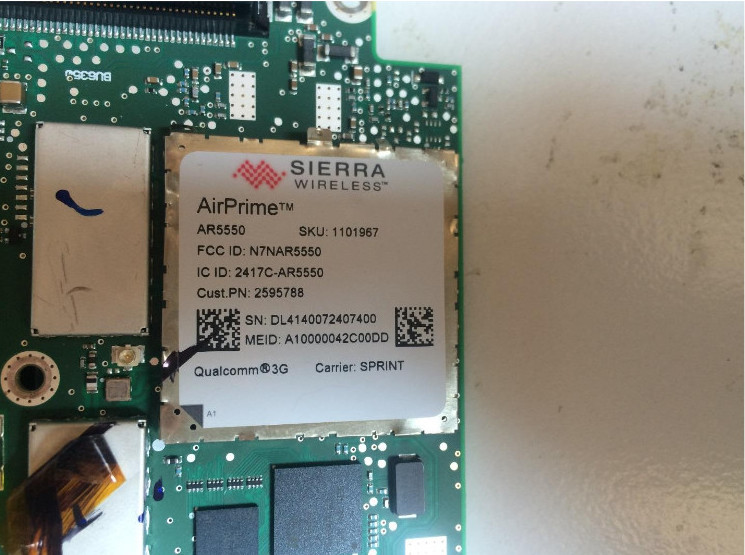
\includegraphics[width=0.3\textwidth]{pic/001_cellular.jpg}
        \caption[Mobilfunk]{Mobilfunk-Einheit im Jeep Cherokee}
        %Sierra Wireless AirPrime AR5550 from a Harman Uconnect system
\cite{Quelle}
%Quelle für Bild:
% [MV15]
\end{figure}


	\end{center}
    \begin{itemize}
		\item
    \end{itemize}

\end{frame}
 \begin{frame}
	\frametitle{Mobilfunk II}
    \begin{itemize}
		\item
    \end{itemize}
\end{frame}


 \subsection{WLAN} % erscheint in Gliederung
 \begin{frame}
	\frametitle{WLAN}
    \begin{itemize}
		\item
    \end{itemize}
\end{frame}
 \subsection{Bluetooth} % erscheint in Gliederung

\begin{frame}
	\frametitle{Bluetooth}
    \begin{itemize}
		\item
    \end{itemize}
\end{frame}

\begin{frame}
	\frametitle{Der Arbeitsbereich Sicherheit in Verteilten Systemen (SVS)}
	\begin{block}{Lorem ipsum dolor}
		Lorem ipsum dolor sit amet, consectetur adipisicing elit, sed do eiusmod tempor incididunt ut labore et dolore magna aliqua. Ut enim ad minim veniam, quis nostrud exercitation ullamco laboris nisi ut aliquip ex ea commodo consequat.
	\end{block}
	\begin{itemize}
		\item Themen
			\begin{enumerate}
				\item Privacy Enhancing Technologies (PET)
				\item Security Management \& Risk Management
				\item Security of Mobile Systems
			\end{enumerate}
		\item Weitere Informationen
			\begin{itemize}
				\item http://www.informatik.uni-hamburg.de/svs
			\end{itemize}
	\end{itemize}
\end{frame}


\begin{frame}
	\frametitle{Beispiel für eine Abbildung}
	\begin{itemize}
		\item Zweck
			\begin{itemize}
				\item Nur mit \alert{berechtigten Partnern} weiter kommunizieren
				\item Verhindert unbefugte Inanspruchnahme von Betriebsmitteln
			\end{itemize}
	\end{itemize}
	\vspace{\fill}
	\pause % Das Nachfolgende erst nach Klick einblenden...
	\begin{center}
		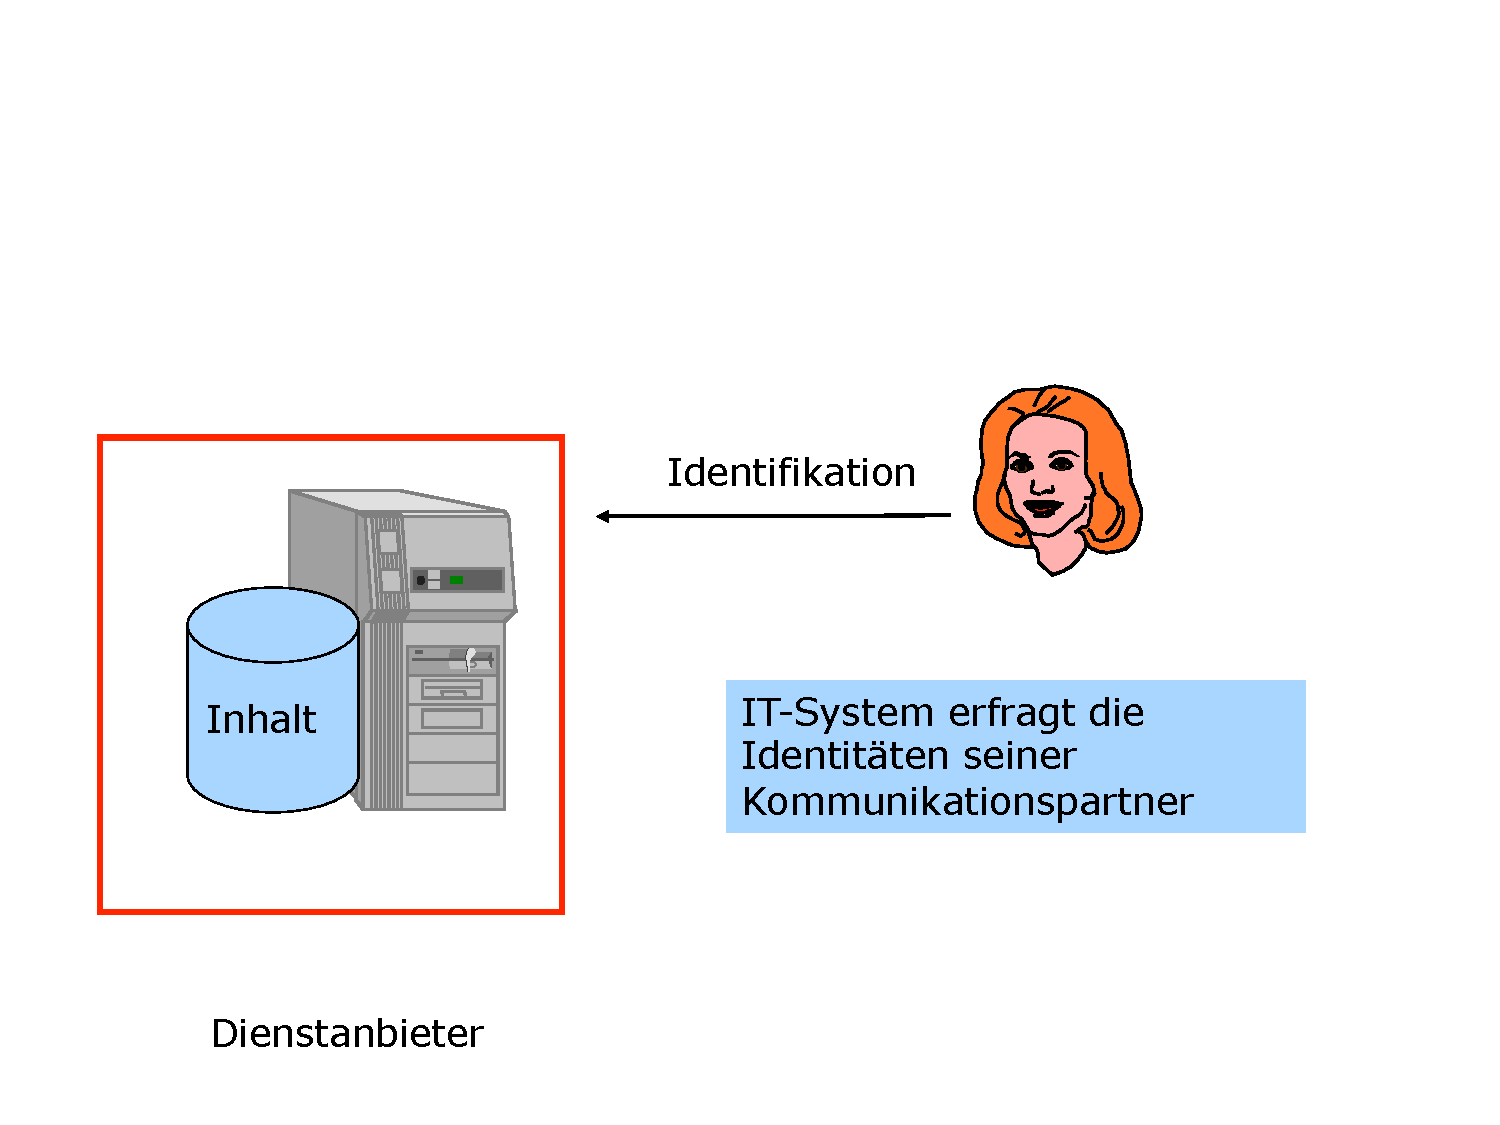
\includegraphics[width=0.8\textwidth]{pic/abbildung1.pdf}
	\end{center}
\end{frame}


\begin{frame}
	\transwipe % funktioniert nur bei Anzeige mit Acrobat Reader
	\frametitle{Beispiel für eine Abbildung}
	\begin{itemize}
		\item Zweck
			\begin{itemize}
				\item Einem Kunden \emph{\color[RGB]{0,128,0} K} einen Inhalt \emph{\color{red} I} in einer bestimmten Weise zugänglich machen, ihn aber daran hindern, \emph{alles} damit tun zu können.
			\end{itemize}
	\end{itemize}
	\vspace{\fill}
	\begin{center}
		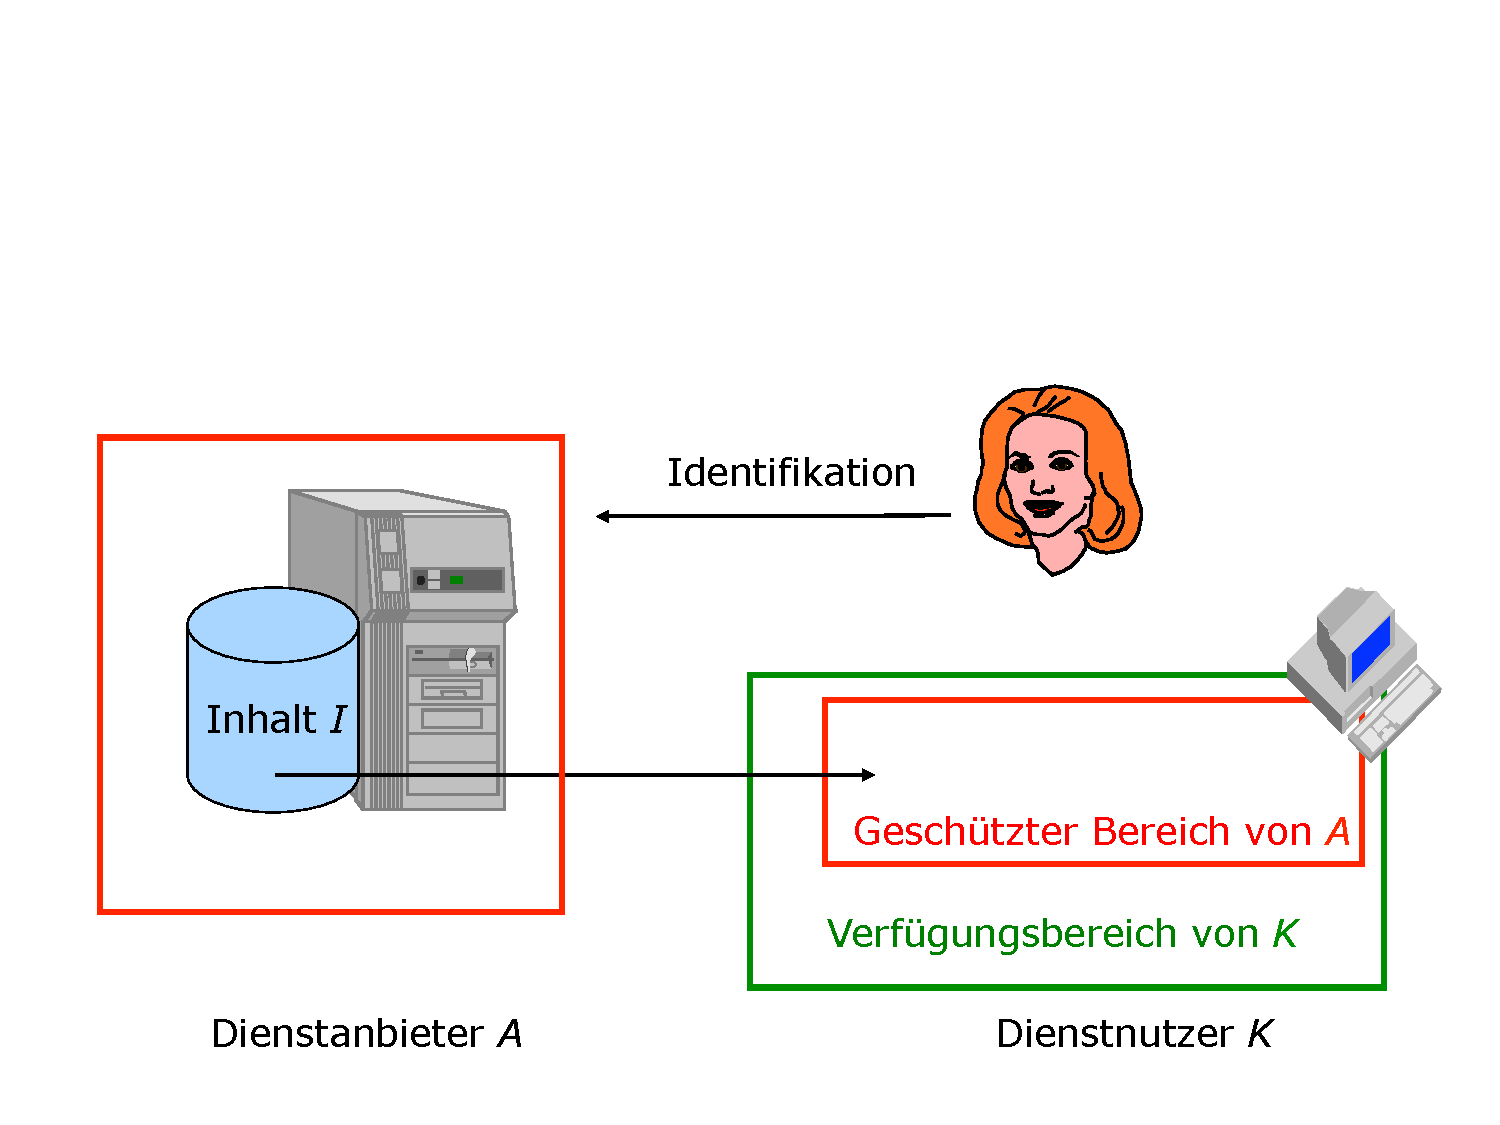
\includegraphics[width=0.8\textwidth]{pic/abbildung2.pdf}
	\end{center}
\end{frame}


\begin{frame}
	\frametitle{Weiteres Beispiel für eine Abbildung}
	\framesubtitle{[John Doe, 1966] }
	\begin{itemize}
		\item Voraussetzung: {\color{black} Angreifer}
			\begin{itemize}
				\item betreibt täuschend echte Webseite der Bank
				\item bewegt den Kunden zum Besuch dieser Seite
			\end{itemize}
	\end{itemize}
	\vspace{\fill}
	\begin{center}
		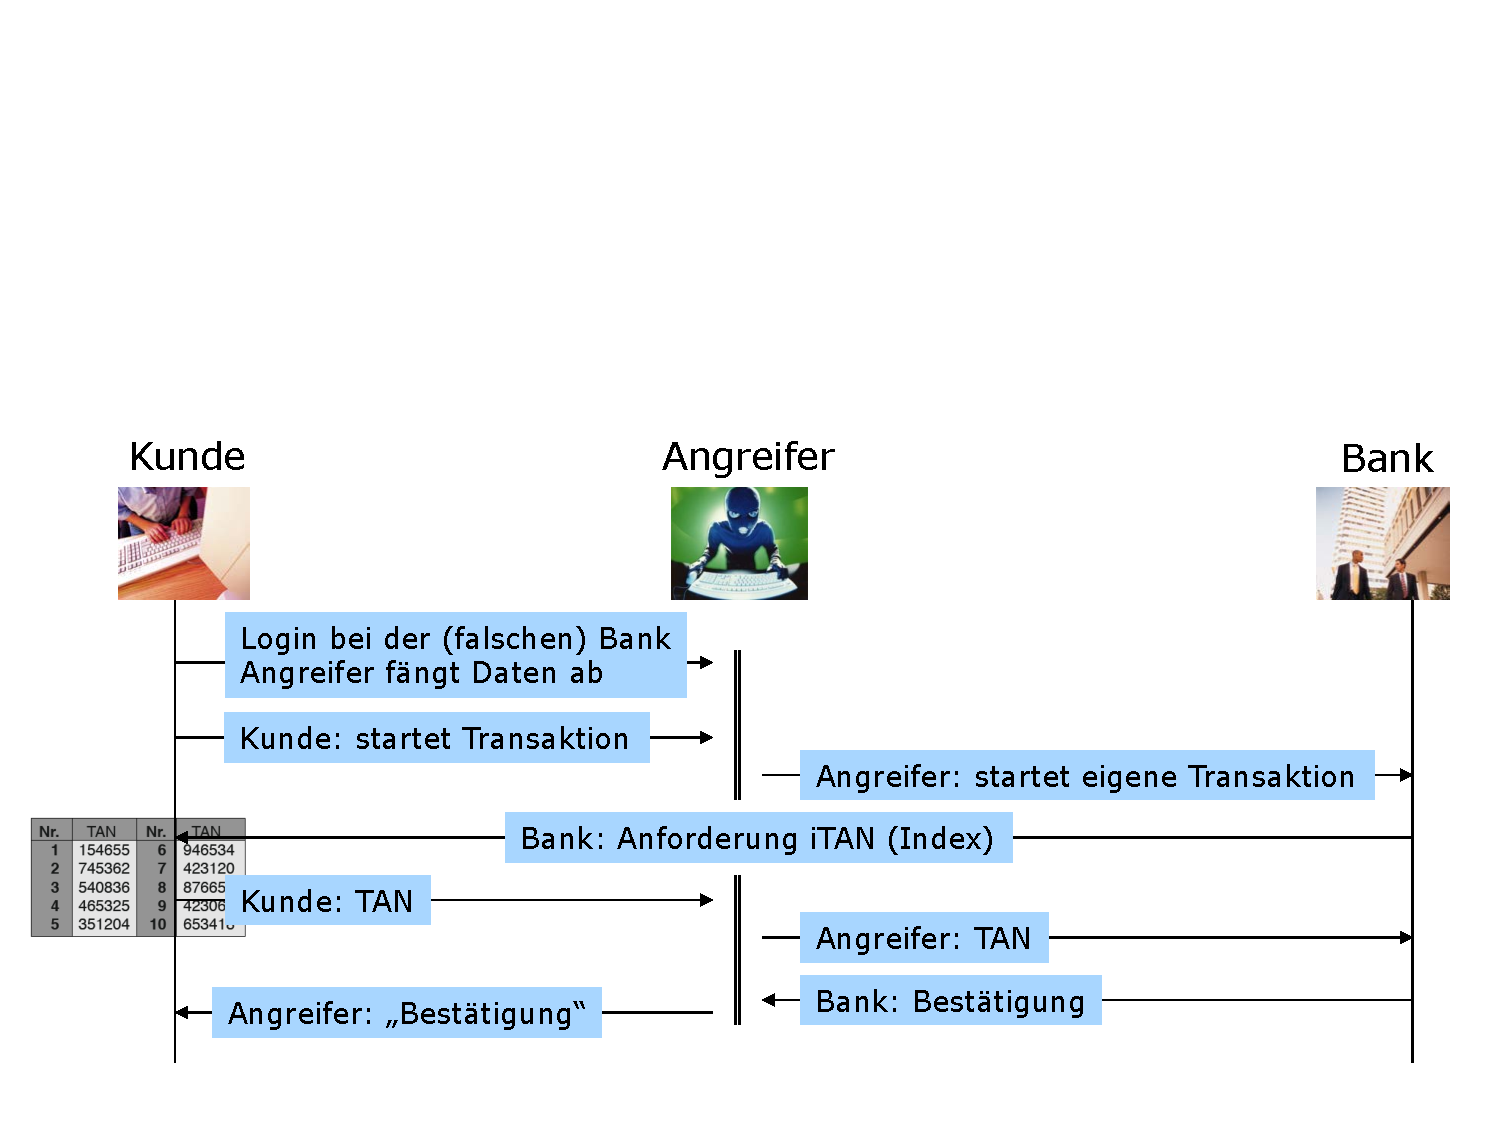
\includegraphics[width=\textwidth]{pic/abbildung3.pdf}
	\end{center}
\end{frame}


\begin{frame}
	\frametitle{Ebenen}
	\begin{itemize}
		\item Erste Ebene
			\begin{itemize}
				\item Zweite Ebene
				\begin{itemize}
					\item Dritte Ebene
				\end{itemize}
				\item Zweite Ebene
			\end{itemize}
		\item Erste Ebene
	\end{itemize}
	\begin{enumerate}
		\item Erste Ebene
			\begin{enumerate}
				\item Zweite Ebene
				\begin{enumerate}
					\item Dritte Ebene
				\end{enumerate}
				\item Zweite Ebene
			\end{enumerate}
		\item Erste Ebene
	\end{enumerate}
\end{frame}


\begin{frame}{Spalten}
	\begin{columns}[T]
		\begin{column}{.6\textwidth}
			\begin{itemize}
				\item Linke Spalte
				\begin{itemize}
					\item Lorem ipsum dolor sit amet,
					\item consectetur adipisicing elit,
					\item sed do eiusmod tempor incididunt ut
					\item labore et dolore magna aliqua.
				\end{itemize}
				\item Erste Ebene
				\begin{itemize}
					\item Zweite Ebene
					\item Zweite Ebene
				\end{itemize}
				\item Erste Ebene
				\begin{itemize}
					\item Zweite Ebene
					\item Zweite Ebene
				\end{itemize}
			\end{itemize}
		\end{column}
		\begin{column}{.4\textwidth}
			\begin{center}
				\vspace{1cm}
				
\includegraphics[width=2.2cm]{pic/svs_logo_hires-ohne-was.png} \\
				Das SVS-Logo
			\end{center}
		\end{column}
	\end{columns}
\end{frame}

\end{document}
